\documentclass[10pt]{article}

\usepackage[a4paper,margin=0.75in,columnsep=0.24in]{geometry}
\usepackage{booktabs}
\usepackage{hyperref}
\usepackage{graphicx}
\usepackage{xcolor}
\usepackage{tikz}
\usepackage{multicol}
\usepackage{caption}
\setlength{\parskip}{0pt}
\usetikzlibrary{arrows.meta, positioning, shapes.geometric}

\newcommand{\todo}[1]{{\color{red}[TODO: #1]}}
\definecolor{edgeblue}{HTML}{2F6FED}
\definecolor{edgegreen}{HTML}{2E8B57}
\definecolor{edgeorange}{HTML}{D9822B}
\definecolor{edgegray}{HTML}{F2F4F8}

\title{ONNX-EdgeIDS: A Lightweight Two-Stage Edge Serving Toolkit for Network Intrusion Detection}
\author{Thai Nguyen Vu \and \todo{Coauthors}}
\date{}

\begin{document}
\maketitle
\vspace{-1.5em}

\begin{abstract}
\small
ONNX-EdgeIDS is a research-software toolkit for deploying machine-learning
network intrusion detection on resource-constrained edge devices. It provides a
Kafka flow replay utility, a first-stage anomaly gate that filters high-volume
traffic, and a second-stage ONNX Runtime classifier node for low-latency
inference on Jetson-class hardware. The package also includes a transparent
NumPy inference backend, artifact export scripts, feature-order checks, and
validation utilities so that researchers can compare exported predictions with a
reference offline model before deployment. ONNX-EdgeIDS turns the limitation of
heavyweight IDS serving stacks into a reusable software contribution: model
training and selection remain offline, while the online path uses portable
artifacts and lightweight runtimes for reproducible throughput, latency, and
load-shedding experiments.
\end{abstract}

\noindent\textbf{Keywords:} Intrusion detection; ONNX Runtime; edge computing;
Kafka; Jetson; research software
\vspace{0.25em}

\section*{Code metadata}
\vspace{-0.6em}
\begin{center}
\footnotesize
\begin{tabular}{p{0.24\textwidth}p{0.70\textwidth}}
\toprule
Current code version & v0.1.0 \\
Repository for this version & \url{https://github.com/vuthainguyen1602/onnx-edge-ids} \\
Reproducible capsule & \todo{Optional Zenodo/Code Ocean link after release archive} \\
Legal code license & MIT \\
Code versioning system used & Git \\
Languages/tools/services & Python, NumPy, ONNX Runtime, Kafka \\
Requirements/dependencies & Python $\geq$ 3.9; NumPy; kafka-python; optional ONNX Runtime; optional artifact-conversion dependencies \\
Documentation/manual & \url{https://github.com/vuthainguyen1602/onnx-edge-ids} \\
Support email & thaivn\_ph@utc.edu.vn \\
\bottomrule
\end{tabular}
\end{center}

\section*{Software metadata}
\vspace{-0.6em}
\begin{center}
\footnotesize
\begin{tabular}{p{0.24\textwidth}p{0.70\textwidth}}
\toprule
Software name & ONNX-EdgeIDS \\
Software type & Edge inference, artifact validation, and load-test software \\
Repository & \url{https://github.com/vuthainguyen1602/onnx-edge-ids} \\
Target users & Researchers and engineers deploying ML-based IDS on edge devices \\
Supported model family in current release & ONNX-compatible binary IDS classifiers; NumPy fallback for tree ensembles \\
Main inputs & Feature metadata, ONNX/NumPy artifact, Kafka flow records \\
Main outputs & Predictions, confidence values, suspicious-flow messages, validation and latency logs \\
Hardware evaluated & NVIDIA Jetson Orin Nano Super; \todo{board/OS} \\
\bottomrule
\end{tabular}
\end{center}

\begin{multicols}{2}

\section{Impact overview}

Machine-learning intrusion detection research often reports classifier accuracy
but leaves deployment behavior hard to reproduce. Edge deployments add a second
problem: the online classifier must process bursts of network flows under memory
and latency limits. ONNX-EdgeIDS addresses this gap by packaging the serving
side of an IDS experiment as reusable software rather than as an ad hoc runtime
script tied to a single training environment.

The software contributes a two-stage architecture for reproducible edge
experiments. A lightweight gate node consumes raw flow records and forwards only
suspicious candidates to a second Kafka topic. A classifier node on a separate
edge device consumes that reduced stream and serves an ONNX artifact. This
separation lets researchers measure the gate hit rate, classifier latency,
end-to-end throughput, and backpressure under controlled traffic replay.

ONNX-EdgeIDS is useful for follow-up work because it treats the model artifact,
feature order, and validation report as part of the software interface. This
reduces the chance that an IDS result is caused by a hidden preprocessing
mismatch, and it makes deployment comparisons possible across CPU ONNX Runtime,
accelerator-backed ONNX providers, and the transparent NumPy backend.

\section{Software description}

ONNX-EdgeIDS contains four main components. The artifact preparation scripts
create ONNX and NumPy serving artifacts and write the feature-column metadata
that fixes the runtime input order. The validation module compares exported
predictions against a reference offline model on replayed flow records and
reports label agreement and confidence differences.


\begin{center}
\scriptsize
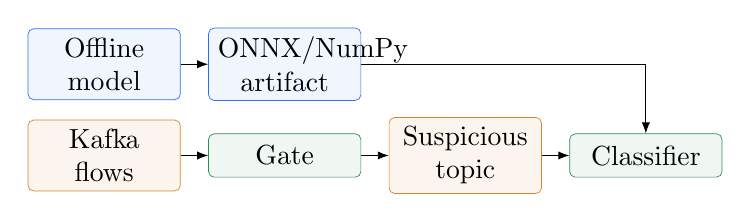
\begin{tikzpicture}[
  node distance=2.5mm and 3.5mm,
  stage/.style={draw, rounded corners=2pt, align=center, minimum height=5.5mm,
    text width=17mm, fill=edgegray, line width=0.25pt},
  blue/.style={stage, draw=edgeblue, fill=edgeblue!7},
  green/.style={stage, draw=edgegreen, fill=edgegreen!7},
  orange/.style={stage, draw=edgeorange, fill=edgeorange!8},
  arrow/.style={-{Latex[length=1.4mm]}, line width=0.35pt}
]
\node[blue] (dev) {Offline\\model};
\node[blue, right=of dev] (art) {ONNX/NumPy\\artifact};
\node[orange, below=of dev] (flow) {Kafka\\flows};
\node[green, right=of flow] (gate) {Gate};
\node[orange, right=of gate] (sus) {Suspicious\\topic};
\node[green, right=of sus] (cls) {Classifier};
\draw[arrow] (dev) -- (art);
\draw[arrow] (art) -| (cls);
\draw[arrow] (flow) -- (gate);
\draw[arrow] (gate) -- (sus);
\draw[arrow] (sus) -- (cls);
\end{tikzpicture}
\captionof{figure}{Two-stage ONNX-EdgeIDS serving path.}
\label{fig:onnx-edgeids-workflow}
\end{center}

The prediction layer exposes a small NumPy-based interface shared by the ONNX
and NumPy backends. This keeps the application code independent from the
training toolchain and allows the same batch of feature vectors to be evaluated
through either backend. The ONNX Runtime backend is the default serving path;
the NumPy backend is intended for debugging, model-inspection, and environments
where ONNX Runtime is not installed.

The Kafka utilities implement the two-stage deployment. The producer replays CSV
flow records to an input topic. The gate node performs fast first-stage
filtering and forwards suspicious records to a second topic. The classifier node
loads the ONNX or NumPy artifact, emits class labels and confidence values, and
records per-message latency so that the deployment can be profiled on one or two
Jetson devices.

\section{Illustrative use case}

The motivating use case is a two-Jetson IDS experiment. Jetson \#1 runs the
Kafka broker and the gate node, while Jetson \#2 runs the classifier node. The
researcher prepares an ONNX artifact from the selected offline IDS model, syncs
the repository and artifacts to both boards, starts the Kafka topics, replays a
traffic CSV, and records throughput and p95 latency from the classifier logs.

\todo{Insert final validation numbers: rows, label agreement, max probability
delta, artifact size.}

\todo{Insert final deployment numbers: gate throughput, classifier throughput,
p95 latency, RAM, and power on the two Jetson boards.}

\section{Limitations and future work}

The current release focuses on binary IDS classifiers and tree-ensemble serving
artifacts. Additional model families require adapter-specific validation before
they should be used for alert thresholds. The present Kafka pipeline measures
inference behavior on replayed flow records rather than on live packet capture.
Future work will add TensorRT-backed ONNX Runtime measurements on Jetson,
additional IDS datasets, and adapters for more model families.

\section*{Acknowledgements}

\todo{Funding and acknowledgements.}

\bibliographystyle{plain}
\bibliography{references}
\end{multicols}

\end{document}
